\chapter{Выполнение задания}

\section{Выбранный язык программирования}

Для реализации алгоритма был выбран язык C++.

\section{Реализация алгоритма}

На листинге \ref{lst:algo} представлен код реализуемого алгоритма.

\begin{lstlisting}[caption={Нечеткий алгоритм кластеризации c-средних}, label={lst:algo}]
    void c_means_clustering(std::vector<std::vector<double>> &cluster_centers, // -1
    std::vector<std::vector<double>> &membership, // -2
    const std::vector<std::vector<double>> &data, // -3
    double m /* -4 */, double convergenceThreshold /* -5 */, double maxIterations /* -6 */)
{
    int iterations = 0;                                                                  // (1)
    double delta = convergenceThreshold + 1.0;                                           // (2)
    while (iterations < maxIterations && delta > convergenceThreshold)                   // (3)
    {
        for (size_t i = 0; i < data.size(); ++i)                                         // (4)
        {
            for (size_t j = 0; j < cluster_centers.size(); ++j)                          // (5)
            {
                double sum = 0.0;                                                        // (6)
                double dist1 = sqrt(pow(data[i][0] - cluster_centers[j][0], 2) +
                                    pow(data[i][1] - cluster_centers[j][1], 2));         // (7)
                for (size_t k = 0; k < cluster_centers.size(); ++k)                      // (8)
                {
                    double dist2 = sqrt(pow(data[i][0] - cluster_centers[k][0], 2) +
                                        pow(data[i][1] - cluster_centers[k][1], 2));     // (9)
                    sum += pow(dist1 / dist2, 2.0 / (m - 1.0));                          // (10)
                }
                membership[i][j] = 1.0 / sum;                                            // (11)
            }
        }
        for (size_t j = 0; j < cluster_centers.size(); ++j)                              // (12)
        {
            double numeratorX = 0.0;                                                     // (13)
            double numeratorY = 0.0;                                                     // (14)
            double denominator = 0.0;                                                    // (15)
            for (size_t i = 0; i < data.size(); ++i)                                     // (16)
            {
                double membershipPowM = pow(membership[i][j], m);                        // (17)
                numeratorX += membershipPowM * data[i][0];                               // (18)
                numeratorY += membershipPowM * data[i][1];                               // (19)
                denominator += membershipPowM;                                           // (20)
            }
            cluster_centers[j] = { numeratorX / denominator, numeratorY / denominator }; // (21)
        }
        std::vector<std::vector<double>> old_cluster_centers = cluster_centers;
        delta = 0.0;
        for (size_t i = 0; i < cluster_centers.size(); ++i)
        {
            delta = sqrt(pow(data[i][0] - old_cluster_centers[i][0], 2) +
                         pow(data[i][1] - cluster_centers[i][1], 2));
        }
        ++iterations;
    }
}
\end{lstlisting}

\section{Графовые модели алгоритмов}

\subsection{Граф управления}

На рисунке \ref{fig:ctrl-graph} показан граф управления программы.

\begin{figure}[H]
    \centering
    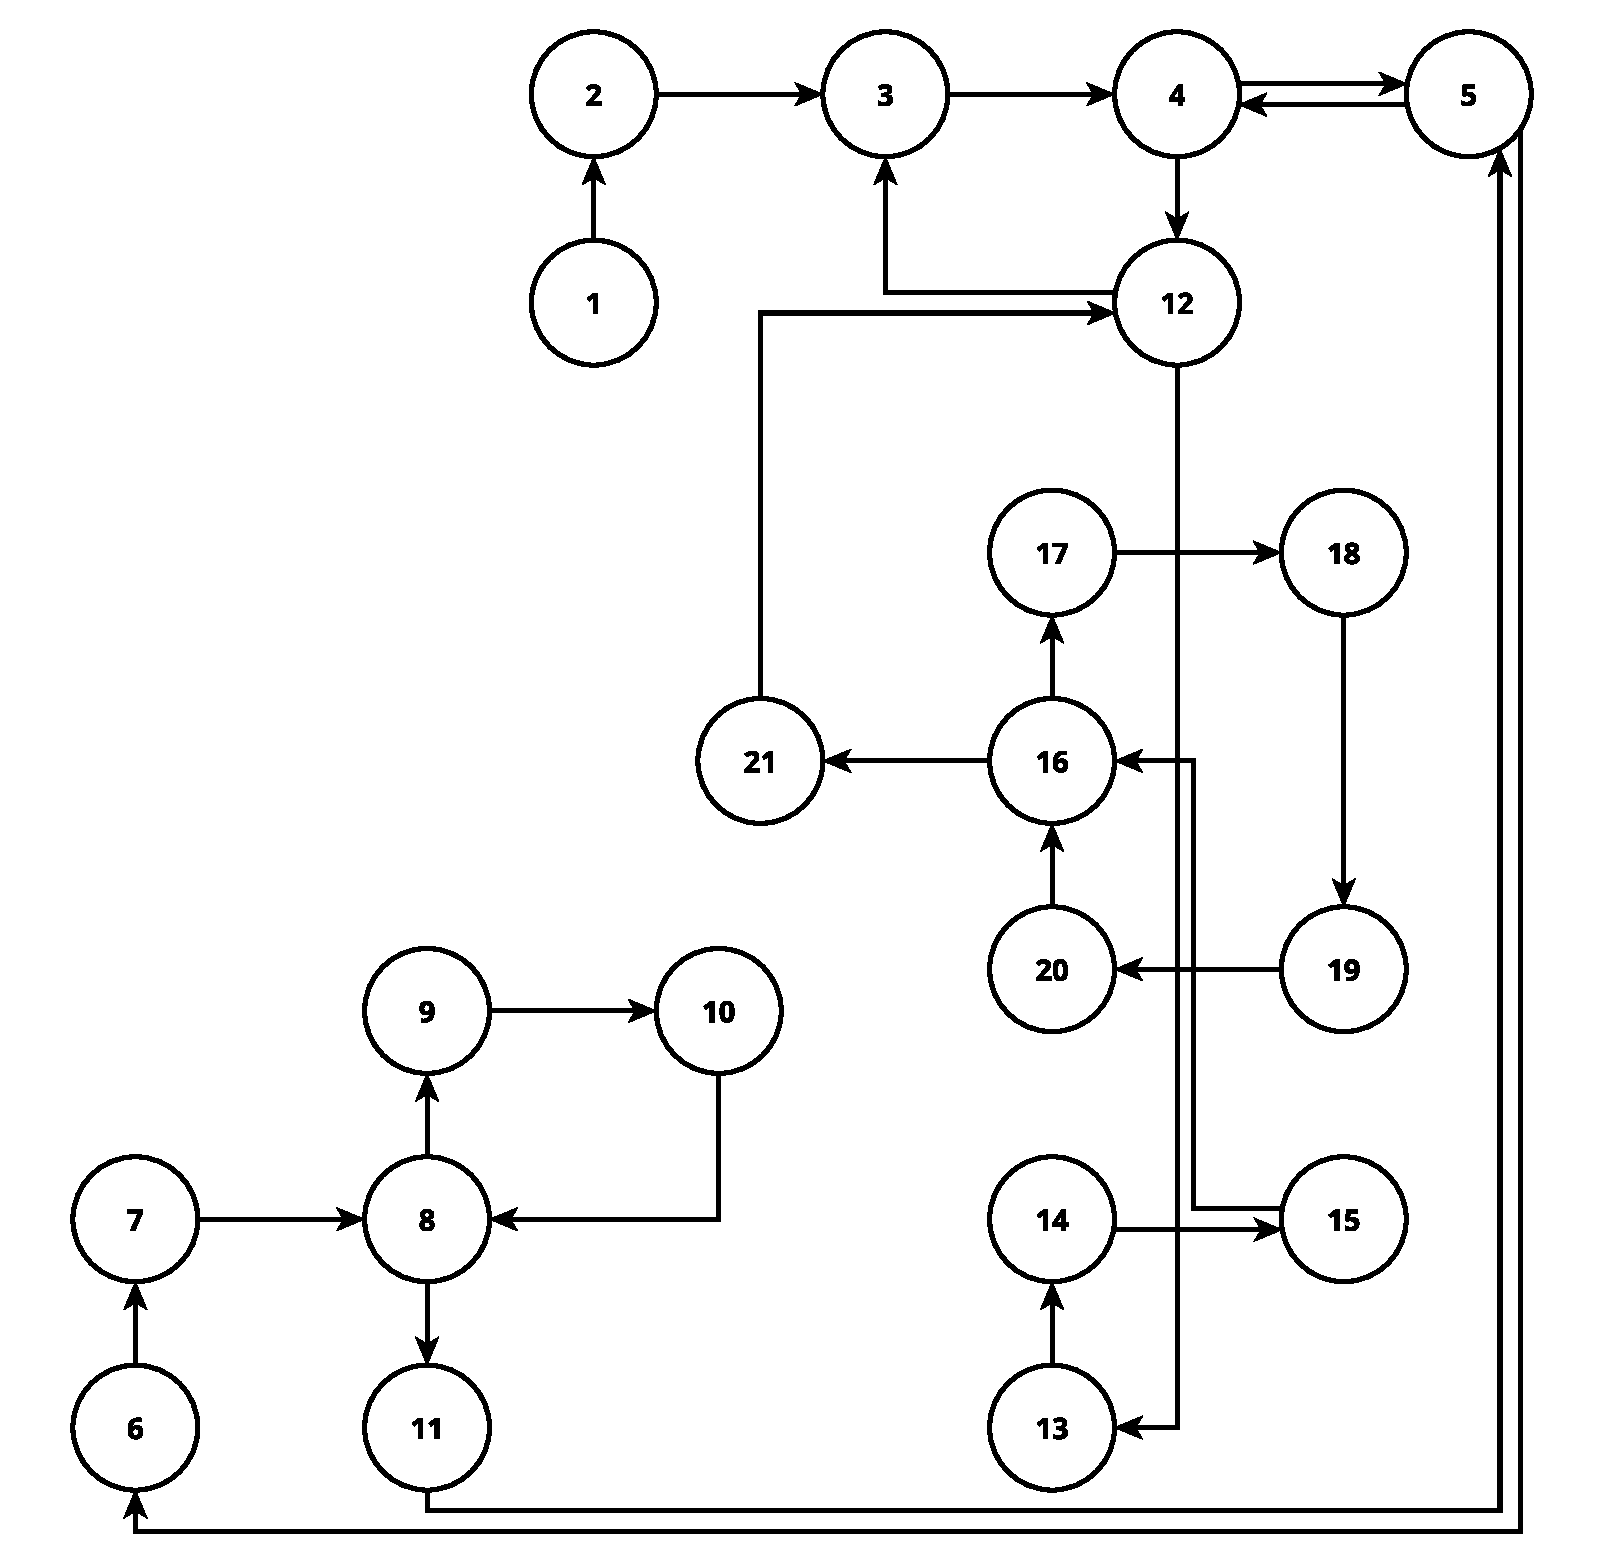
\includegraphics[width=1.0\textwidth, pages=-]{images/control_graph.pdf}
    \caption{Граф управления}
    \label{fig:ctrl-graph}
\end{figure}

\subsection{Информационный граф}

На рисунке \ref{fig:info-graph} представлен информационный граф программы.

\begin{figure}[H]
    \centering
    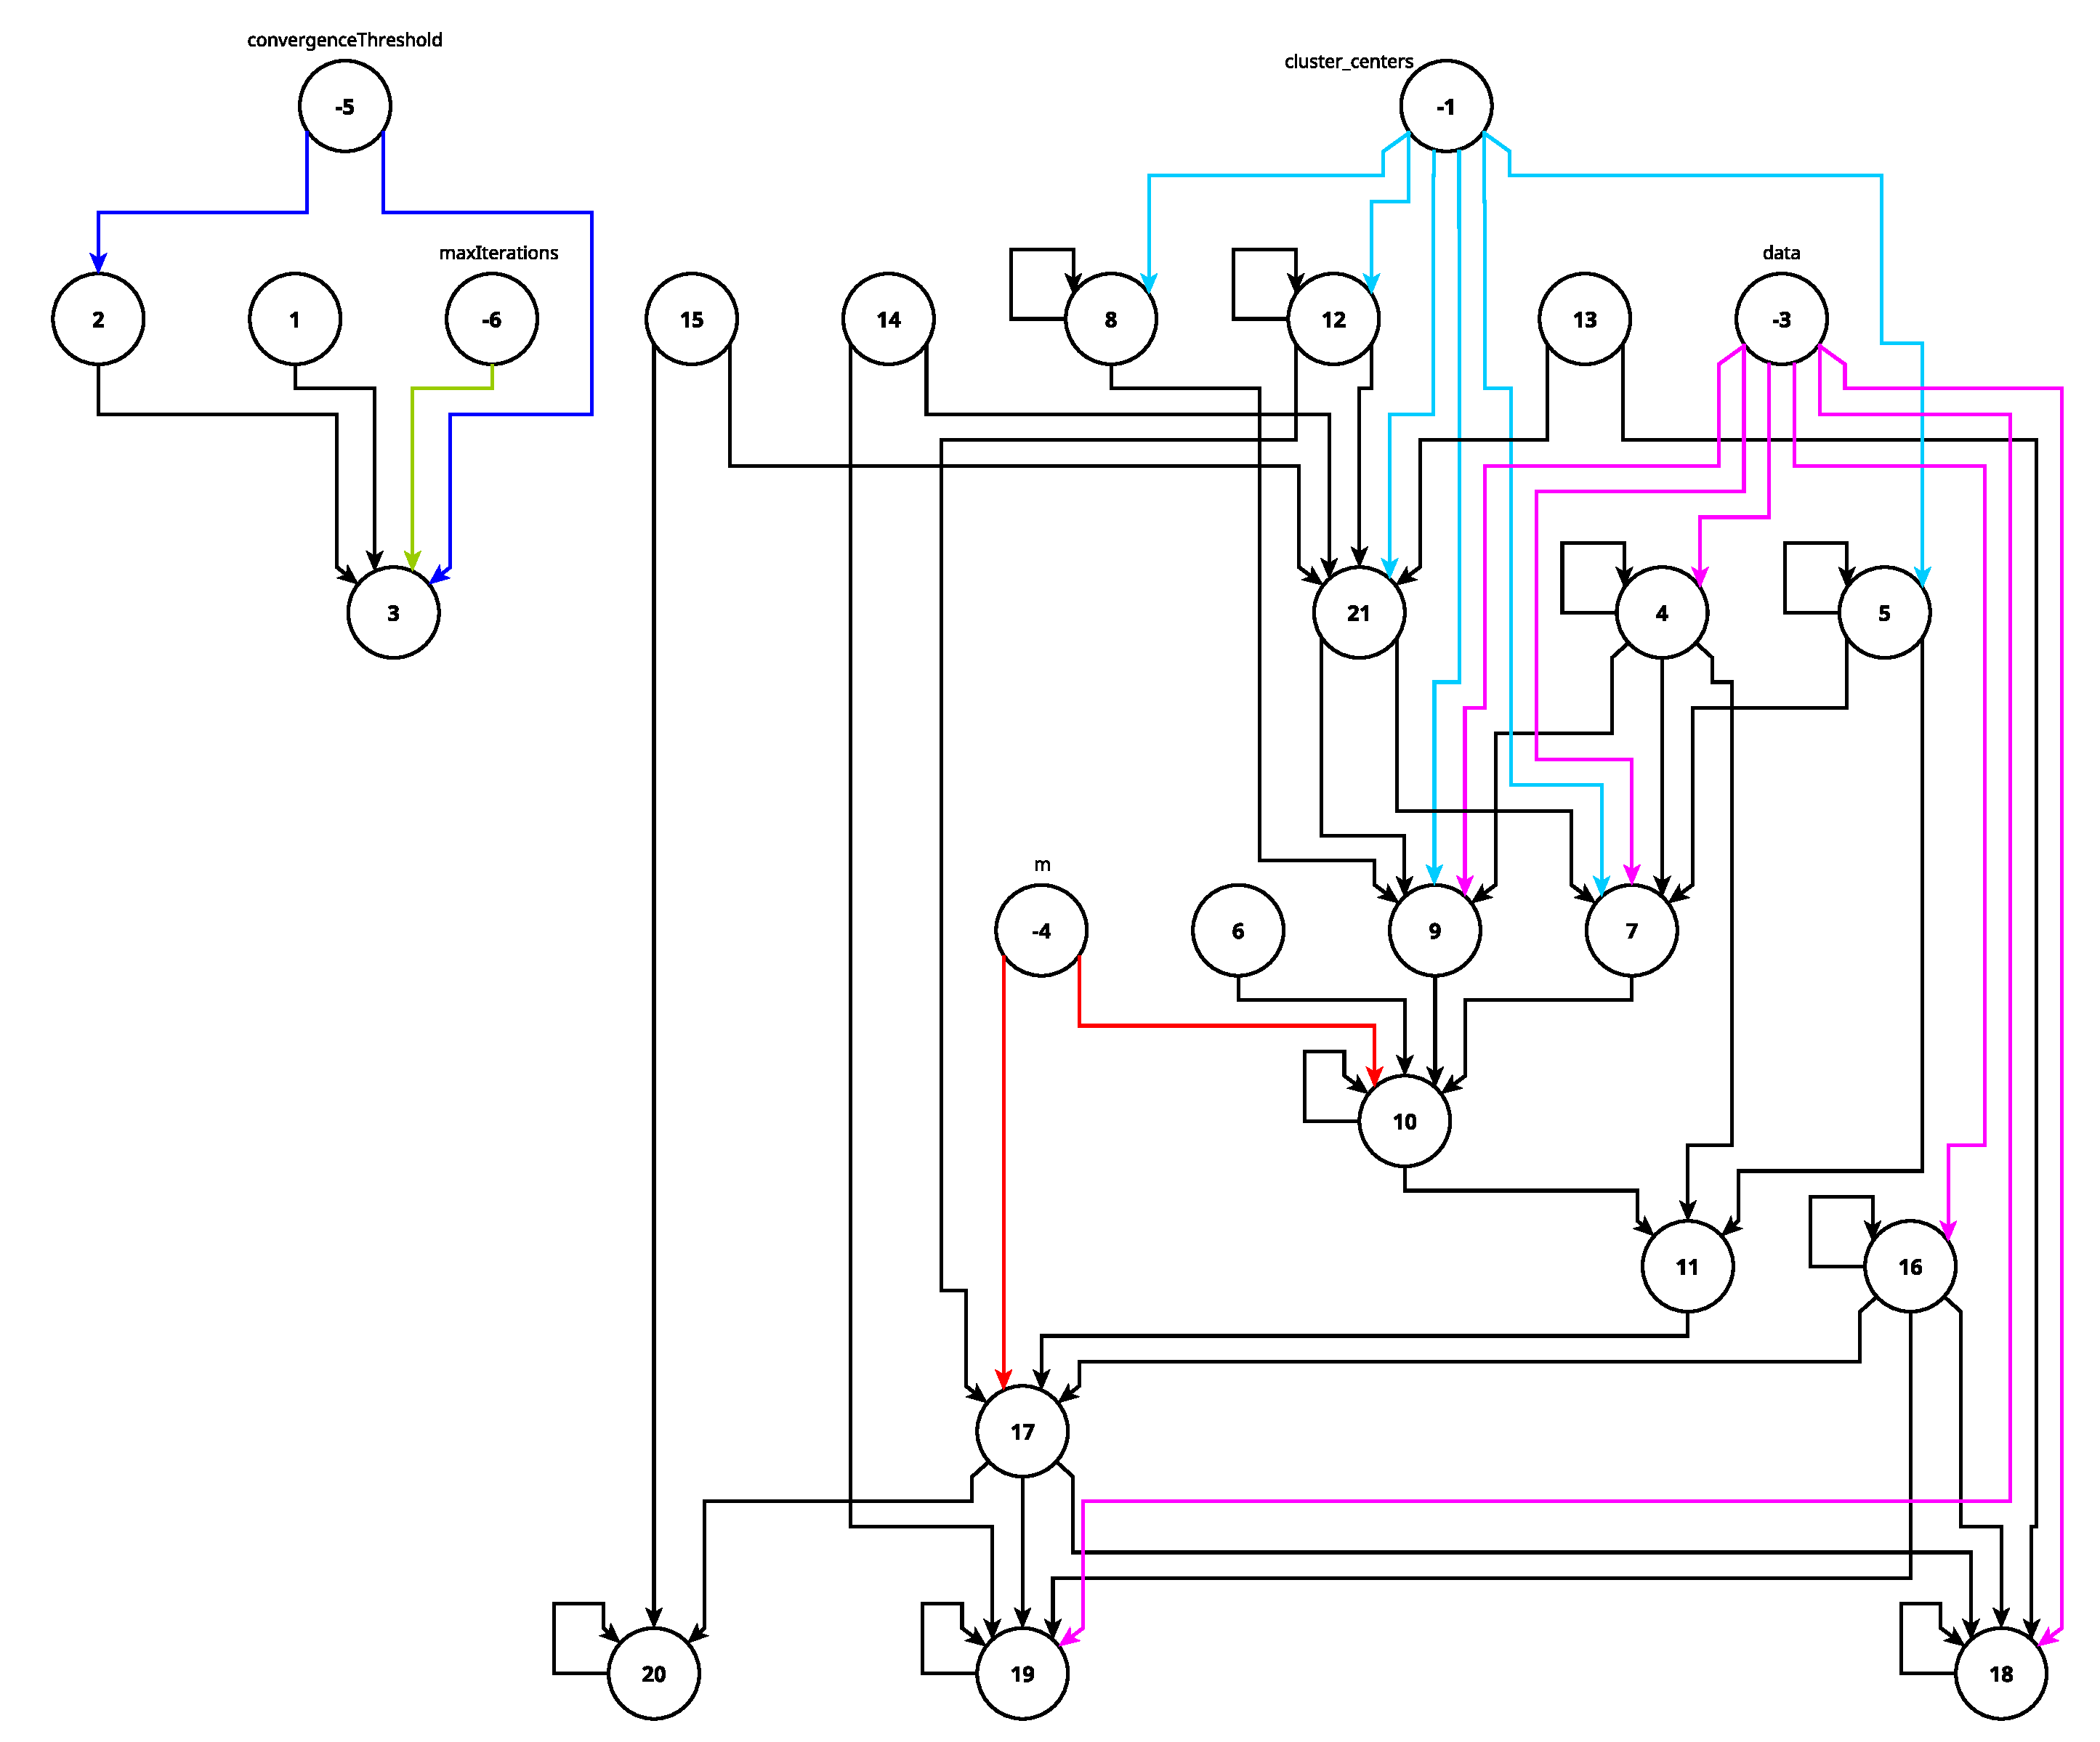
\includegraphics[width=1.0\textwidth, pages=-]{images/info_graph.pdf}
    \caption{Информационный граф}
    \label{fig:info-graph}
\end{figure}

\subsection{Операционная история}

Операционная история программы представлена на рисунке \ref{fig:ctrl-graph} для следующих входных данных:
\begin{itemize}
    \item \texttt{k = 1};
    \item \texttt{m = 2};
    \item \texttt{maxIterations = 2};
    \item \texttt{convergenceThreshold = 0.1};
    \item \texttt{data = [[5.1, 2.5], [1.4, 0.2]]}.
\end{itemize}
Для этих же данных будет составлена операционная история.

\begin{figure}[H]
    \centering
    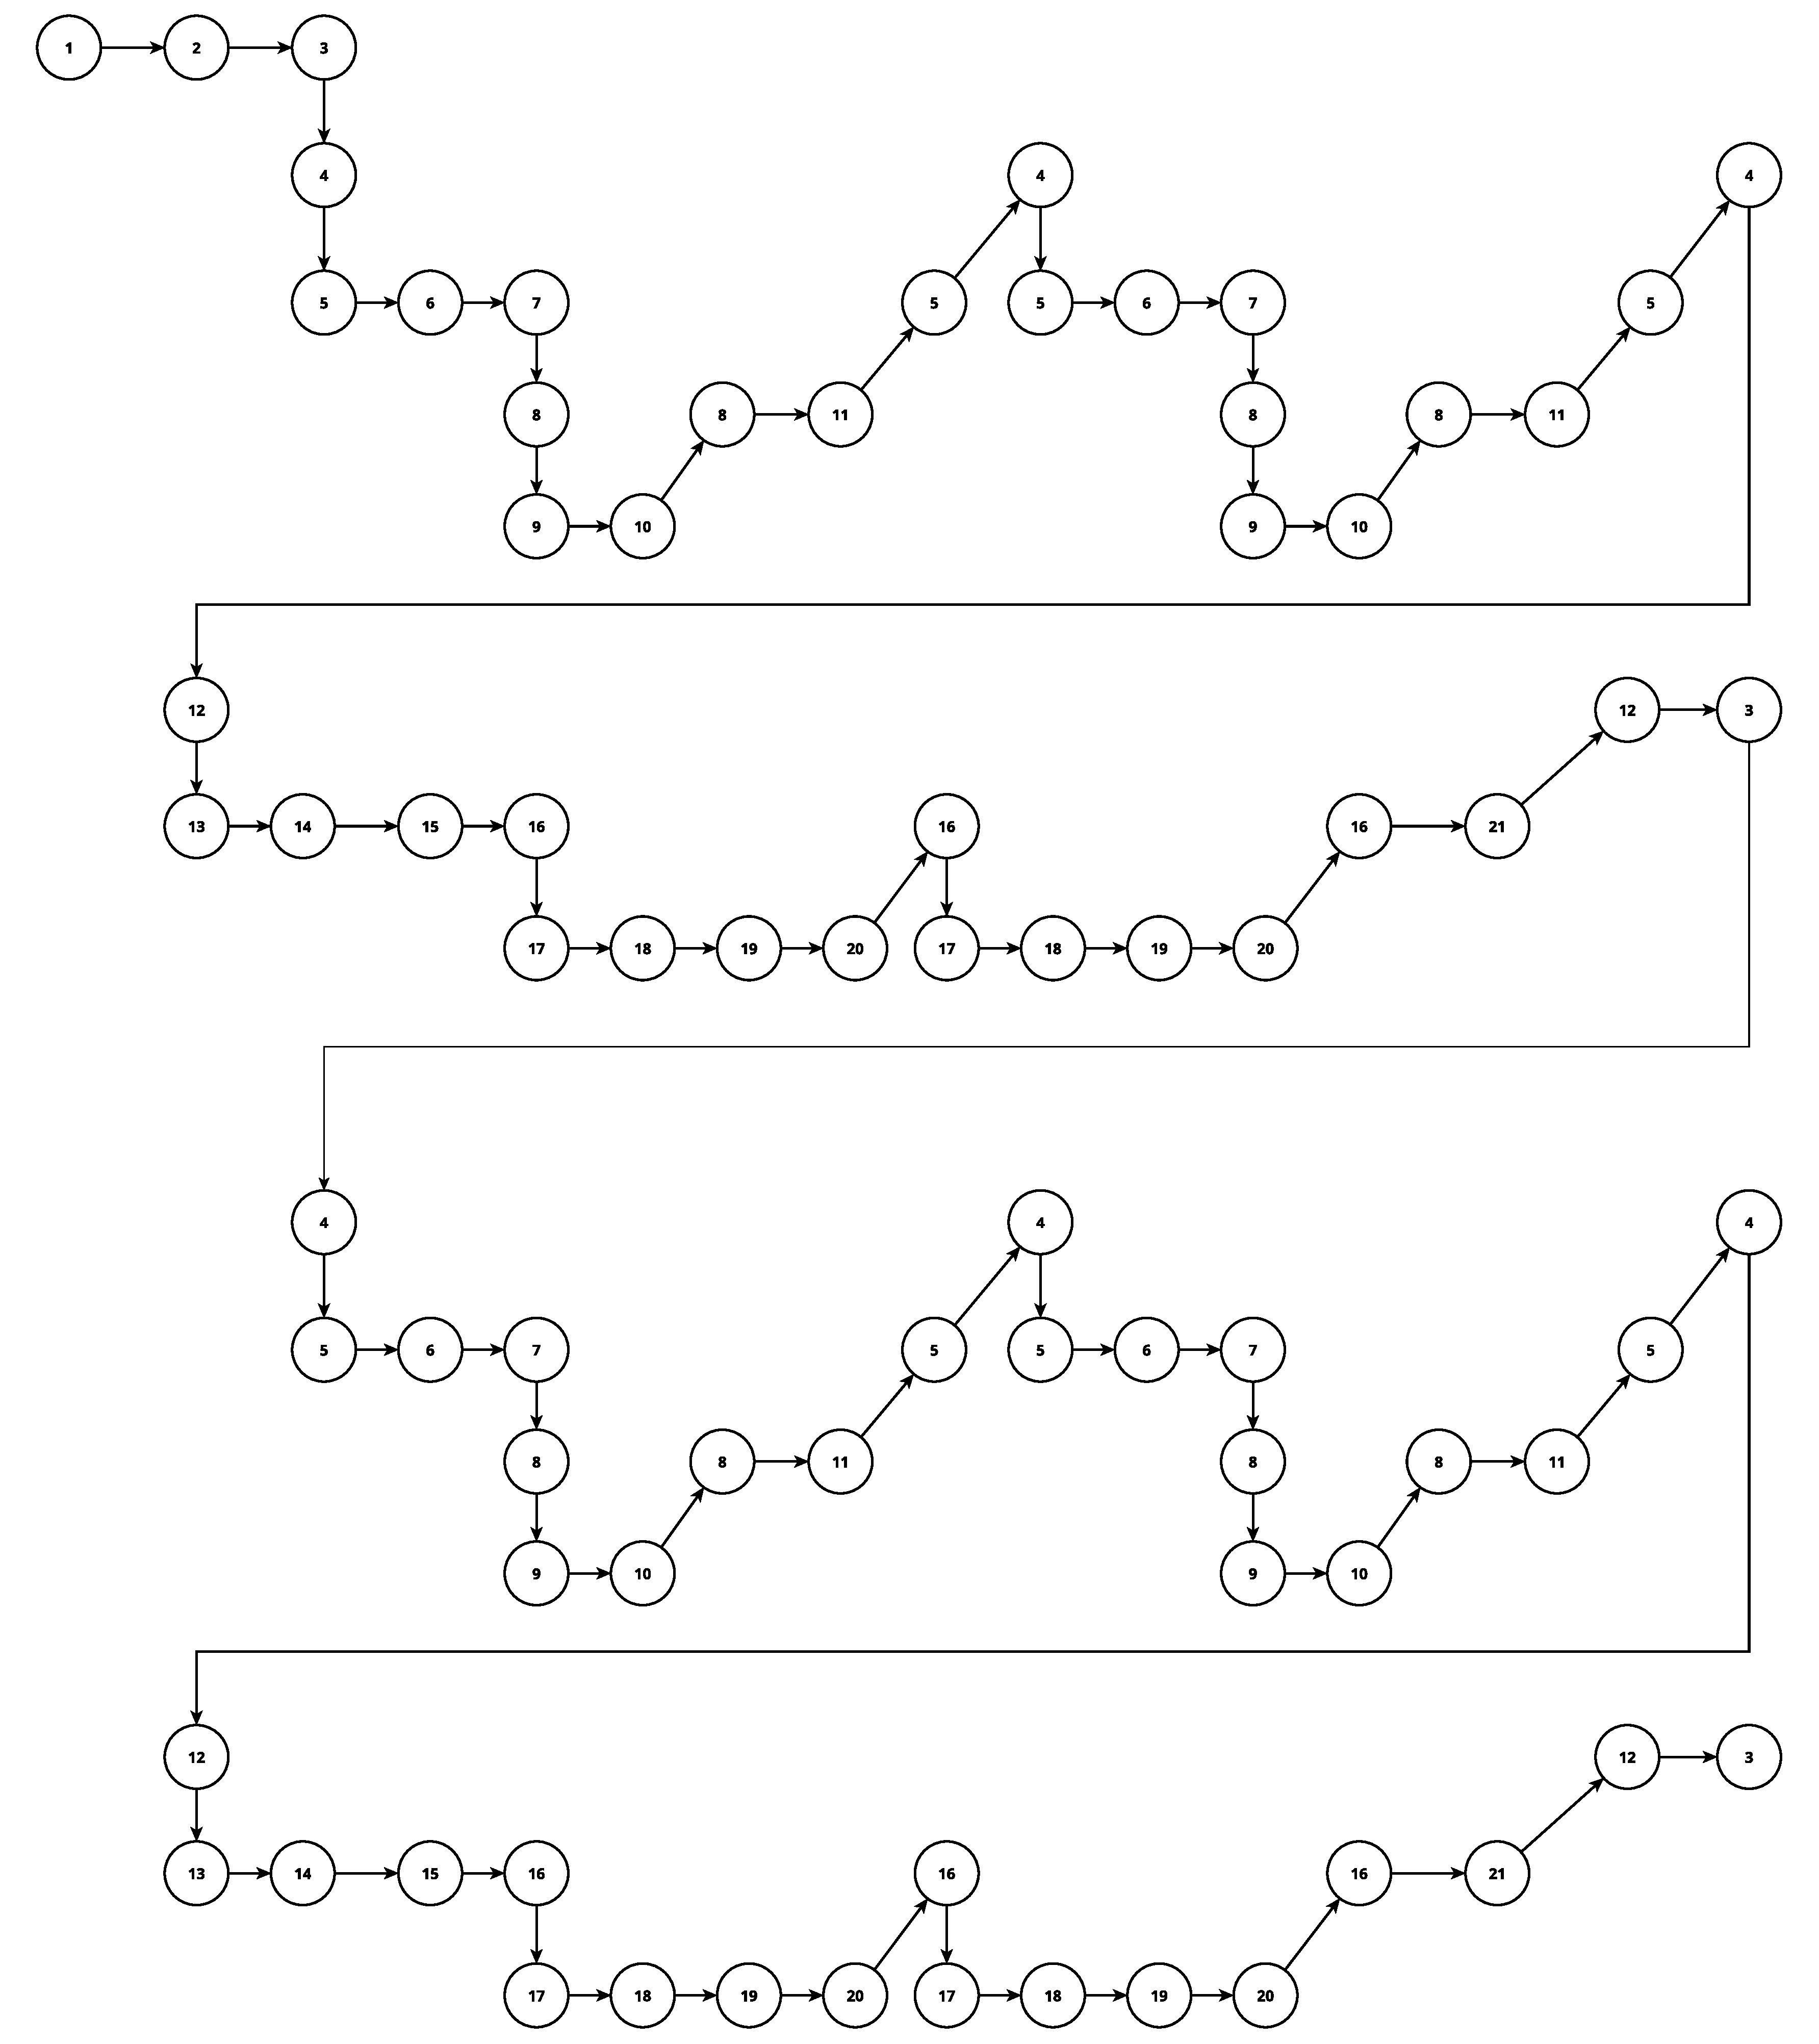
\includegraphics[width=1.0\textwidth, pages=-]{images/op_history.pdf}
    \caption{Операционная история}
    \label{fig:op-hist-graph}
\end{figure}

\subsection{Информационная история}

На рисунке \ref{fig:info-hist-graph} представлена информационная история работы программы.

\begin{figure}[H]
    \centering
    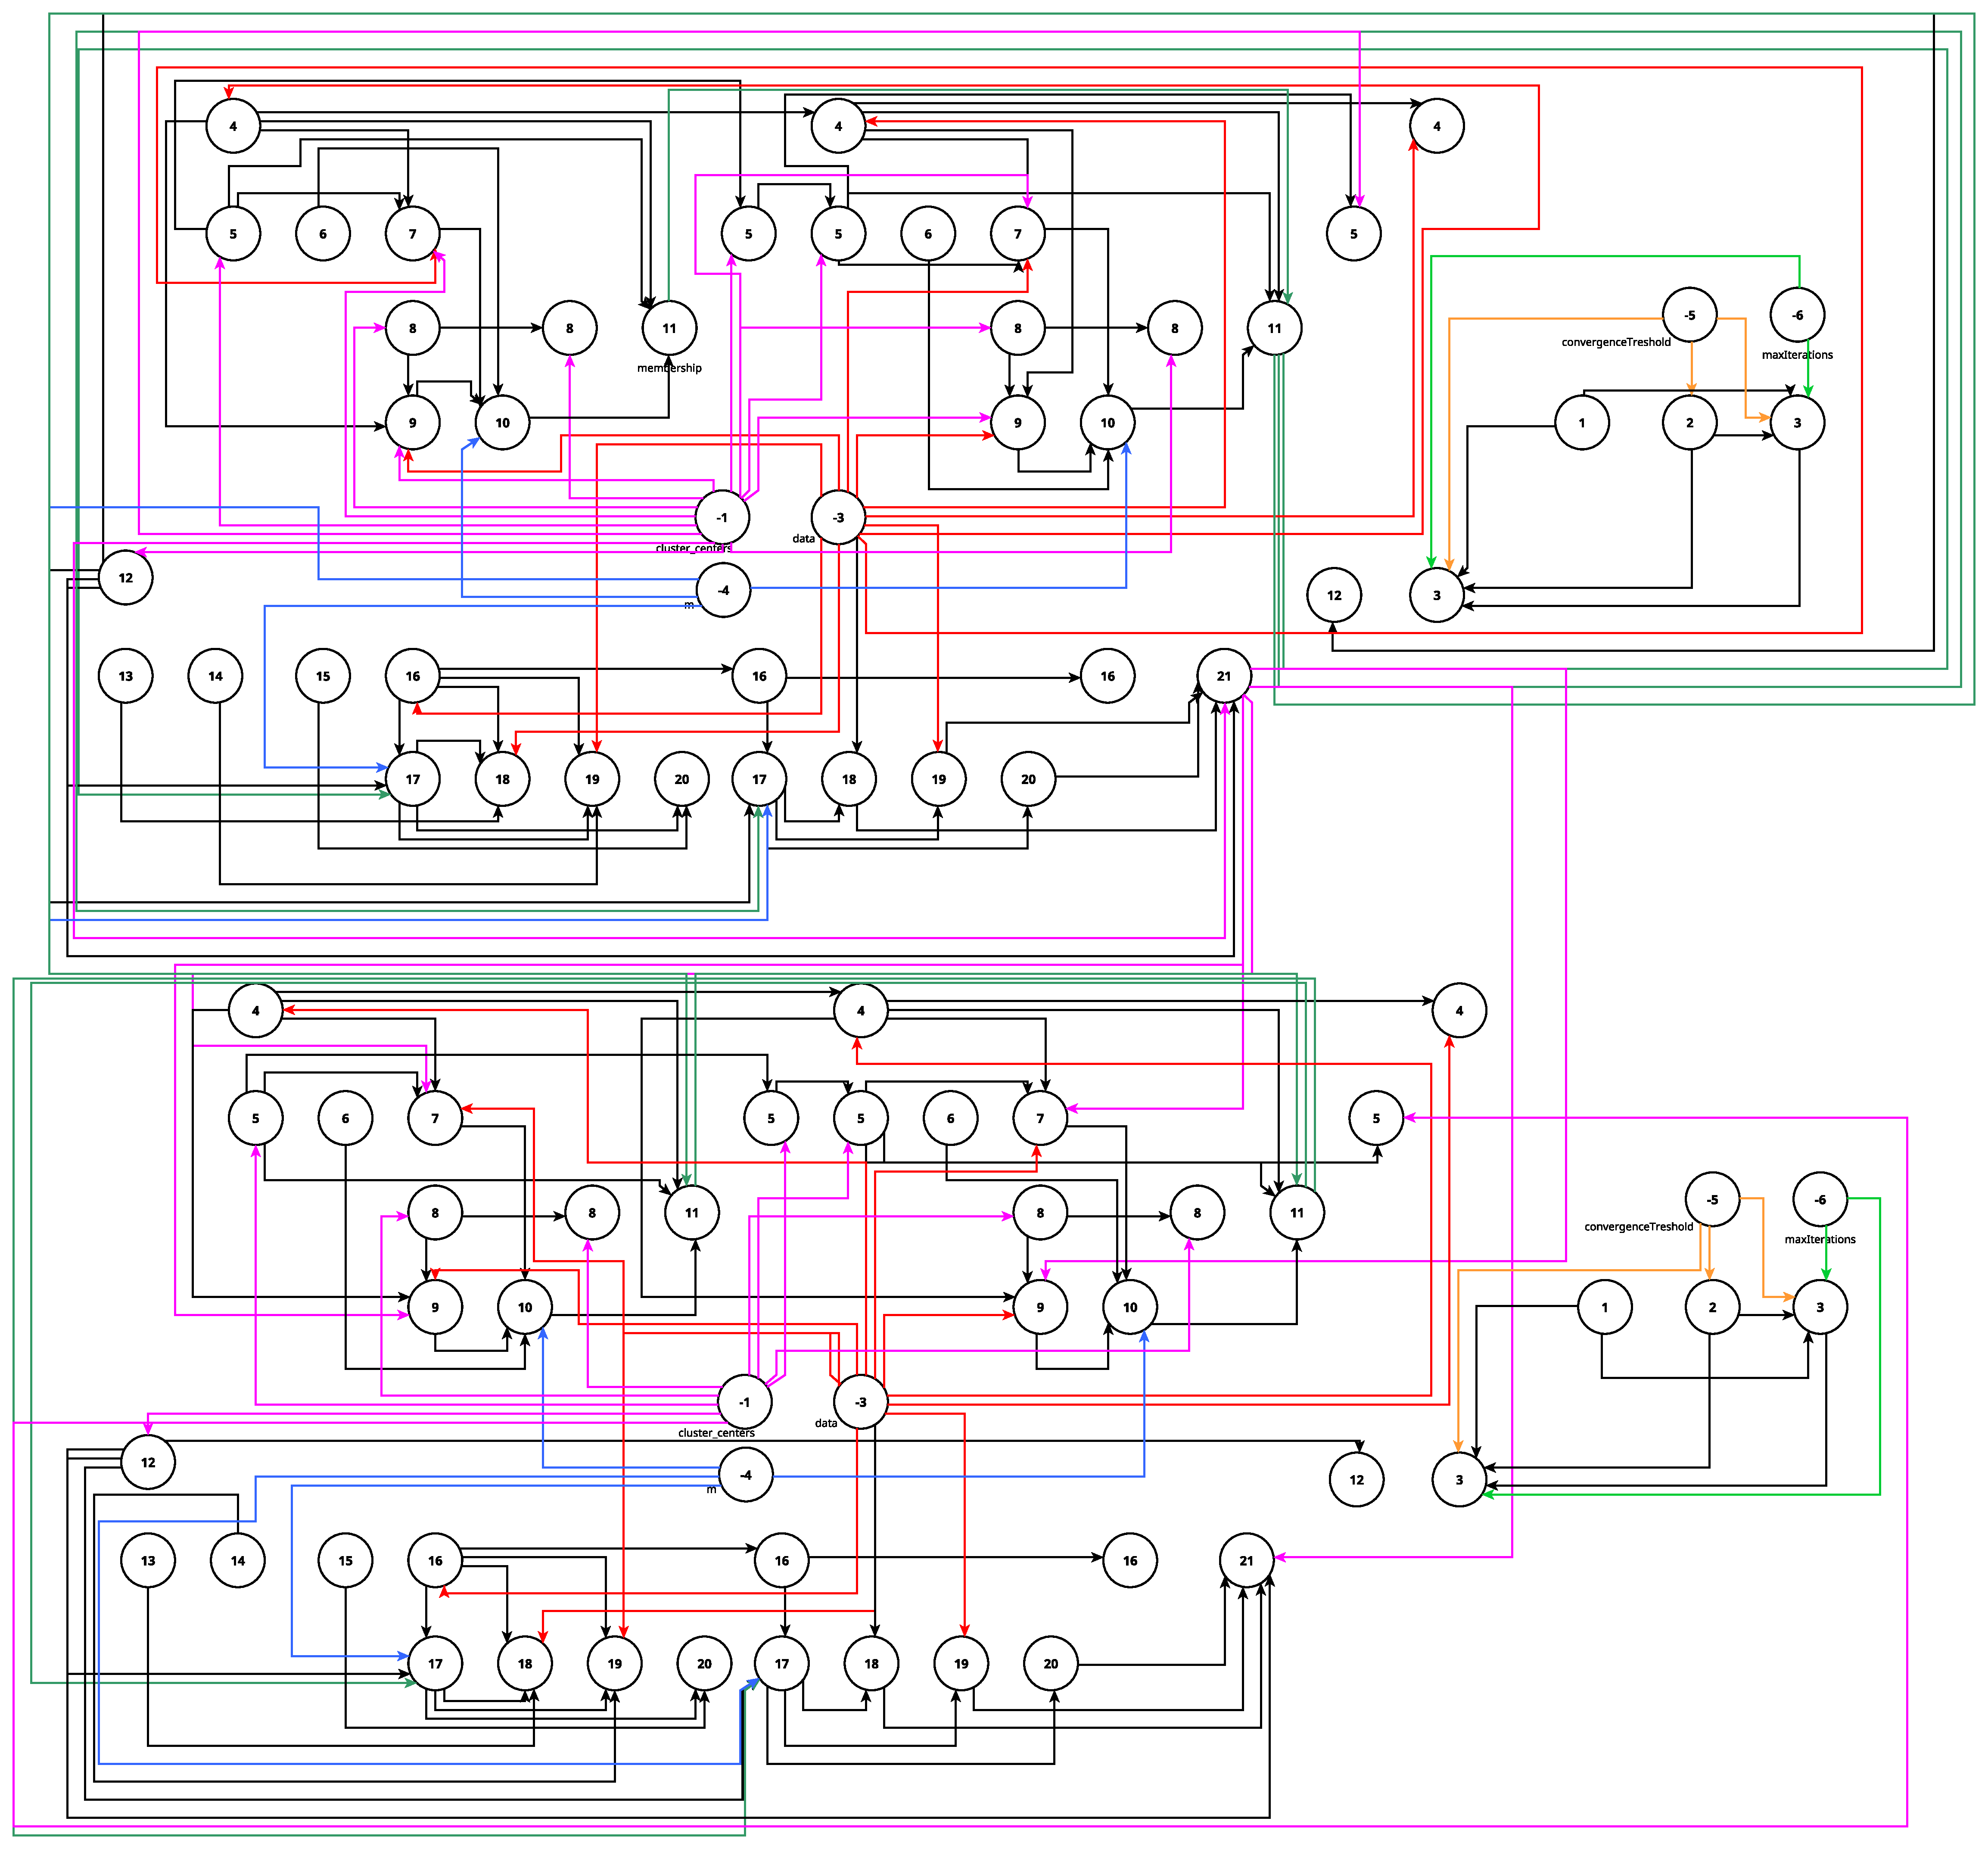
\includegraphics[width=1.0\textwidth, pages=-]{images/info_history.pdf}
    \caption{Информационная история}
    \label{fig:info-hist-graph}
\end{figure}

\chapter*{Возможность распараллеливания}
\addcontentsline{toc}{chapter}{Возможность распараллеливания}

Алгоритм кластеризации c-средних может быть распараллелен следующими способами:
\begin{itemize}
    \item параллельная инициализация центроидов;
    \item параллельное обновление центроидов после кластеризации.
\end{itemize}